\documentclass[titlepage,landscape]{seminar}
\usepackage{url}
\usepackage{graphicx}
\usepackage[pdftex]{color}
\usepackage{hyperref}
\usepackage{epstopdf}
\usepackage{slides}

\newcommand{\frack}{\frac{1}{k}}

\begin{document}

\myslide{
\begin{eqnarray}
\frack\sum p_i^2 &=& \bar p^2 + F_{st}\bar p \bar q \label{eq:p2-f} \\
\frack\sum 2p_iq_i &=& 2\bar p\bar q(1 - F_{st}) \label{eq:2pq-f} \\
\frack\sum q_i^2   &=& \bar q^2 + F_{st}\bar p \bar q \label{eq:q2-f}
\end{eqnarray}
\vfill
\[
F_{st} = \frac{\mbox{Var}(p)}{\bar p \bar q}
\]
}

\myslide{
\begin{center}
\begin{tabular}{c|rrr|c}
\hline\hline
           & \multicolumn{3}{c|}{Genotype} & \\
Population & $A_{1}A_{1}$ & $A_{1}A_{2}$ & $A_{2}A_{2}$ & $\hat p$ \\
\hline
Yackeyackine Soak     & 29 & 0 & 0 & 1.0000 \\
Gnarlbine Rock        & 14 & 3 & 3 & 0.7750 \\
Boorabbin             & 15 & 2 & 3 & 0.8000 \\
Bullabulling          & 9  & 0 & 0 & 1.0000 \\
Mt. Caudan            & 9  & 0 & 0 & 1.0000 \\
Victoria Rock         & 23 & 5 & 2 & 0.8500 \\
Yellowdine            & 23 & 3 & 4 & 0.8167 \\
Wargangering          & 29 & 3 & 1 & 0.9242 \\
Wagga Rock            & 5  & 0 & 0 & 1.0000 \\
``Iron Knob Major''   & 1  & 0 & 0 & 1.0000 \\
Rainy Rocks           & 0  & 1 & 0 & 0.5000 \\
``Rainy Rocks Major'' & 1  & 0 & 0 & 1.0000 \\
\hline
\end{tabular}
\end{center}
}

\myslide{
\begin{eqnarray*}
\mbox{E}(k) &=& \sum_{k=1}^n k \mbox{P}(k) \\
     &=& n p \quad , \\
\end{eqnarray*}
\begin{eqnarray*}
\mbox{E}(\hat p) &=& \mbox{E}\left(\sum_{k=1}^n (k/n)\right) \\
          &=& \sum_{k=1}^n (k/n) P(k) \\
          &=& (1/n)\left(\sum_{k=1}^n k P(k)\right) \\
          &=& (1/n)(n p) \\
          &=& p \quad . \\
\end{eqnarray*}
}

\myslide{
\begin{eqnarray*}
\mbox{E}(\tilde H) &=& \mbox{E}\left(2\hat p (1 - \hat p)\right) \\
     &=& 2\left(\mbox{E}(\hat p) - \mbox{E}({\hat p}^2)\right) \\
     &=& \mbox{TAMO} \\
     &=& ((n-1)/n)2p(1-p) \quad . \\
\end{eqnarray*}
}

\myslide{
Nei's $G_{ST}$
\begin{eqnarray*}
H_{i} &=& 1 - {1 \over N} \sum_{k=1}^{N} \sum_{i=1}^{m} {X_{kii}} \\
H_{s} &=& {\tilde n \over {\tilde n - 1}}
         \left[1 - \sum_{i=1}^{m} {\bar {\hat x_{i}^{2}}}
         - {H_{I} \over {2 \tilde n}}\right] \\
H_{t} &=& 1 - \sum_{i=1}^{m} {\bar x_{i}^{2}} + {H_{S} \over {\tilde n}}
         - {H_{I} \over {2 \tilde n N}}
\end{eqnarray*}

\vfill

\[
G_{st} = 1 - \frac{H_i}{h_t}
\]
}

\myslide{
\begin{itemize}

\item {\it Statistical sampling} - Repeated samples from the same
  population differ from one another. For example, the sample
  frequency of an allele, $\hat p$, will differ from sample to sample
  even if the ``true'' population frequency, $p$, is always the same. 

\item {\it Genetic (or evolutionary) sampling} - We are rarely, if
  ever, interested only in the populations or loci we sampled. We are
  almost always interested in using them as ``representatives'' of all
  populations or loci that could have been sampled. In other words the
  populations and loci we actually studied are best regarded as a
  sample from the set of all comparable populations and loci that
  could have been studied.

\end{itemize}
}

\myslide{
\begin{center}
\resizebox{!}{\textheight}{\includegraphics{sampling.eps}}
\end{center}
}

\myslide{
{\bf Weir \& Cockerham's $\theta$}

$x_{mn,i} = 1$ if allele $m$ from individual $n$ is of type $i$ and is
0 otherwise.

\begin{eqnarray*}
\hat p_i &=& \frac{1}{2N}\sum_{m=1}^2\sum_{n=1}^Nx_{mn,i} \\
E(\hat p_i) &=& p_i
\end{eqnarray*}
Assuming that alleles are sampled independently from the population
\begin{eqnarray*}
E(x^2_{mn,i}) &=& p_i \\
E(x_{mn,i}x_{mn',i}) &=& p_i^2 + \sigma_{x_{mn,i}x_{m'n',i}} \\
&=& p_i^2 + p_i(1-p_i)\theta \\
\theta &=& F_{st}
\end{eqnarray*}
}

\myslide{
\begin{center}
  \begin{tabular}{c|ccc}
\hline\hline
Method & $F_{is}$ & $F_{st}$ & $F_{it}$ \\
\hline
Direct            & 0.1372 & 0.2143 & 0.3221 \\
Nei               & 0.3092 & 0.2395 & 0.4746 \\
Weir \& Cockerham & 0.5398 & 0.0387 & 0.5577 \\
\hline
\end{tabular}
\end{center}
\vfill
\begin{center}
\begin{tabular}{cc}
\hline\hline
\multicolumn{2}{c}{Notation} \\
Wright & Weir \& Cockerham \\
\hline
$F_{it}$ & $F$ \\
$F_{is}$ & $f$ \\
$F_{st}$ & $\theta$ \\
\hline
\end{tabular}
\end{center}
}

\myslide{
\begin{eqnarray*}
n_{11,i} &=& \hbox{\# of $A_1A_1$ genotypes} \\
n_{12,i} &=& \hbox{\# of $A_1A_2$ genotypes} \\
n_{22,i} &=& \hbox{\# of $A_2A_2$ genotypes} \\
i         &=& \hbox{population index} \\
I         &=& \hbox{number of populations} \\
\end{eqnarray*}
\begin{eqnarray*}
x_{11,i} &=& p_{i}^2 + fp_{i}(1-p_{i}) \\
x_{12,i} &=& 2p_{i}(1-p_{i})(1-f) \\
x_{22,i} &=& (1-p_{i})^2 + fp_{i}(1-p_{i})
\end{eqnarray*}
}

\myslide{
\[
P({\bf n}|{\bf p},f) \propto \prod_{i=1}^I x_{11,i}^{n_{11,i}}
x_{12,i}^{n_{12,i}} x_{22,i}^{n_{22,i}}
\]
\begin{eqnarray*}
\mbox{P}(f) &=& U(0,1) \\
\mbox{P}(p) &=& \mbox{Beta}(\pi, \theta) \\
\mbox{E}(p_{ik}) &=& \pi \\
\mbox{Var}(p_{ik}) &=& \pi(1-\pi)\theta \\
\theta &=& F_{st}
\end{eqnarray*}
}

\myslide{
\begin{center}
\resizebox{!}{\textheight}{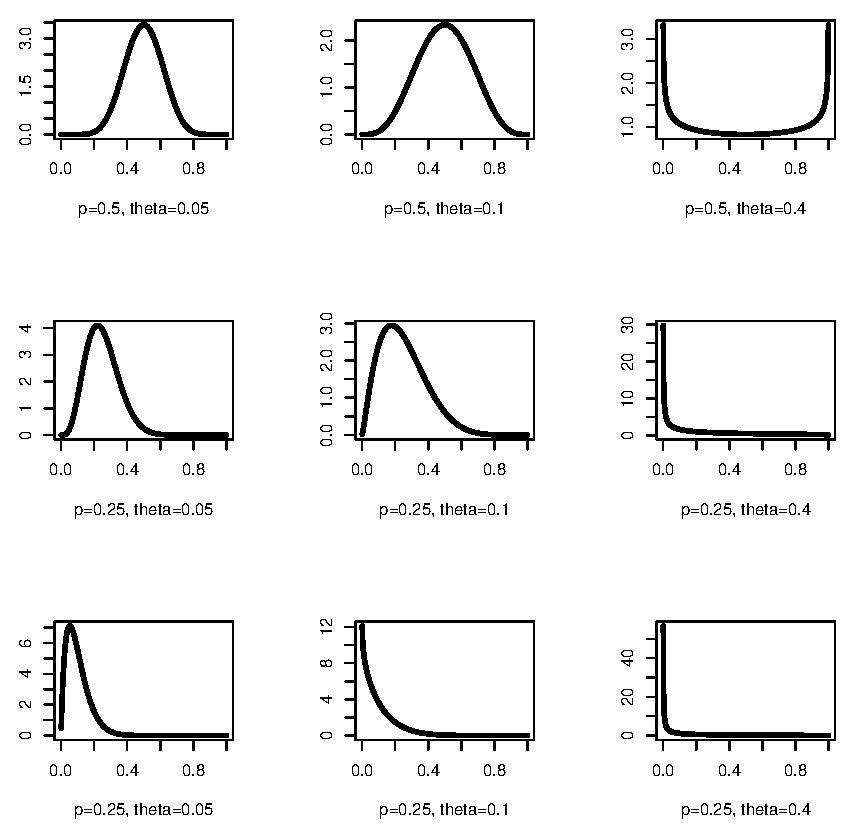
\includegraphics{beta-distribution.eps}}
\end{center}
}

\myslide{
\begin{center}
\begin{tabular}{cccc}
\hline\hline
           &             & \multicolumn{2}{c}{Credible Interval} \\
Parameter  & Mean (s.d.)     & 2.5\% & 97.5\% \\
\hline
$f$            & 0.52 (0.10) & 0.32 & 0.70 \\
$\theta$ & 0.19 (0.12) & 0.03 & 0.50 \\
\hline
\end{tabular}
\end{center}
}

\myslide{
\begin{center}
\begin{tabular}{l|rrrr}
\hline\hline
Model & {\tt Dbar} & {\tt Dhat} & {\tt pD} & {\tt DIC} \\
\hline
Full  & 46.5 & 40.7 & 5.8 & 52.3 \\
$f=0$ & 73.0 & 67.6 & 5.3 & 73.8 \\
$\theta=0$ & 61.6 & 59.8 & 1.8 & 63.5 \\
\hline
\end{tabular}
\end{center}
}

\myslide{
\begin{center}
\begin{tabular}{c|ccc}
\hline\hline
Method & $F_{is}$ & $F_{st}$ \\
\hline
Direct            & 0.14 & 0.21 & 0.32 \\
Nei               & 0.31 & 0.24 & 0.47 \\
Weir \& Cockerham & 0.54 & 0.04 & 0.56 \\
Bayesian          & 0.53 (0.33, 0.70) & 0.11 (0.02, 0.22) \\
\hline
\end{tabular}
\end{center}
}


\end{document}

